
\chapter{Løsning}\label{ch:losning}

\section{Kravspecifikation}
Kravspecifikationen har til formål, at danne grundlag for udviklingen af problemløsningen. Den skal dermed beskrive den ideelle løsning af det analyserede problem samt specificere, hvilke funktioner denne løsning skal indeholde. Herved bliver der enighed om hvilke funktioner der skal implementeres, sådan at listen af funktioner ikke skal udbygges mens projektet skrider frem. Kravene til en løsning, skal desuden overholde en række retningslinjer, der skal sikre at kravspecifikationen er let forståelig og ikke kan misfortolkes. Kravene til kravspecifikationen er beskrevet nedenfor.\\ %Det er derfor vigtigt at hvert krav kun har én betydning. Dermed skal et hvert krav utvetydigt forklarer kravet. Derudover må der ikke være konflikter mellem kravene.

 \noindent \textbf{Entydig} - Kravene skal være entydige, da der ellers kan opstå tvivl om, hvad de forskellige krav betyder. Udover betydningen af kravene, kan formuleringen af kravene, også skabe tvivl hos udviklerne, hvis ikke det er helt klart, hvad der præcist menes. \\

\noindent \textbf{Fuldstændig} - Kravene skal sikre fuldstændighed ved at udfylde alle de punkter, som er specificeret i indholdsfortegnelsen uden at indeholde information, som ikke er relevant for punktet.\\

\noindent \textbf{Konsistent} - Kravene skal være konsistente, hvilket betyder, at der ikke er konflikter mellem kravene. Her skelnes der mellem to former for konflikter. Flere krav der beskriver samme problem under forskellige formuleringer, samt direkte konflikter imellem krav.\\

\noindent \textbf{Korrekt} - Kravene skal være mulige at opfylde og skal være defineret med de rigtige enheder, sådan at et umuligt krav ikke eksisterer.\\

\noindent \textbf{Testbar} - For at opnå en brugbar kravspecifikation, kræves det at kravspecikationen er testbar. En kravspecifikation er testbar når det klart fremgår hvad kravspecifiktationen består af. En testbar kravspecifikation skal også kunne udføres rent økonomisk.\\

\noindent \textbf{Modificerbar} - En brugbar kravspecifikation kræves at være modificerbar, dvs. at det skal være let at tilføje eller ændre krav.\\

\noindent \textbf{Sporbar} - Kravspecifikationen skal være sporbar, hvilket betyder at alle krav skal have en tydelig baggrund i foregående analyse af problemet. \\

%Alle kravene er blevet udarbejdet udfra de foretagede interviews samt , hvor de væsentligste punkter blev trukket ud, samt at kravene ligger vægt på hvad interviewpersonerne satte pris på ved deres løsning. Derudover er der også ved teknologivurderingen blevet fundet mangler ved nuværende løsninger, hvorfor de også er kommet med i kravsspecifikationen.

%Med baggrund i teorien ovenfor er der blevet formuleret en kravspecifikation som opstiller de krav som blev fundet i problemanalysen. Disse er opstillet og danner ramme for en ideel løsning af problemet. Det er ikke muligt inden for den gældende projektperiode at udfylde hele kravspecifikationen og projektgruppen har derfor fokuseret på at overholde en række krav.

Projekt gruppen har forsøgt at efterleve disse kriterier ved at \todo{Sætning stopper. Vi kunne eventuelt bruge noget af det ud kommenteret -Luca}

\subsection{Krav}
Med baggrund i analyse kapitlet er det muligt at opstille en række krav til en ideel løsning af problemet. Disse krav tager baggrund i de fordele og ulemper, som blev fundet i de foretagede interviews samt fordele og egenskaber, som blev fundet i teknologivurderingen. Disse krav beskriver derved en ideel løsning, som projektgruppen har afgrænset sig fra grundet projektperioden. Afgrænsningen kan findes nedenfor kravene.
\begin{itemize}
    \item \textbf{Kapacitet}: Op til 50 medarbejdere, skal kunne være brugere i systemet, da der tages udgangspunkt i små virksomheder. Dette kommer af definitionen på SMV, som er på max 50 mennesker \ref{SMV}.
    \item \textbf{Time registrering}: Systemet skal tælle medarbejderens arbejdstimer, så lederen har mulighed for at se, hvor meget den enkelte medarbejder arbejder.
    \item \textbf{Løn registrering}: Systemet skal ved hjælp af time registreringen styre lønnen. Her skal lederen have mulighed for at indsætte et skema over takster for en given dag, som bruges til at udregne den enkelte medarbejders løn ud fra vedkommendes timeantal. Medarbejderen skal også selv have mulighed for at se deres antal af løntimer løbende, så de ved hvor meget de har indtjent med de gældende takster nedsat af lederen.
    \item \textbf{Arbjedslov}: Det skal være muligt for lederen af vælge om systemet skal advare i tilfælde af overskridelser af de forskellige love og regler i henhold til arbejdsmiljøloven, samt fagforening. %eventuelt i form af en advarsels, eller en automatisk konktaktelese til arbejdstilsynet i forbindelse med overtrædelse af loven.
    \item \textbf{Kategorisering}: Lederen skal have mulighed for at oprette kategorier over arbejdsvagttyperne, som finder sted på arbejdspladsen. For hver medarbejder skal det ligeledes afgøres hvilke arbejdsvagtstyper personen kan tage. Derved kan systemet forhindre medarbejdere i at bytte vagter, hvis ikke medarbejderen som modtager vagten er kvalificeret til at tage denne arbejdsvagtstype.
    \item \textbf{Mobil app}: Systemet skal have en tilhørende app, som medarbejderne kan benytte til at se og bytte vagter. Dette vil give løsningen større tilgængelighed.
    \item \textbf{Server}: Systemet benytter en server, som henter og gemmer data fra en database. Brugeren af programmet skal derfor først logge ind på den virksomhed de arbejder på, hvorefter der vil blive sendt en besked ud til den tilhørende database. Systemet kan herved implementeres til nye virksomheder, ved at tilføje dem til serveren.
    \item \textbf{Kontaktliste}: Kontaktoplysninger om alle medarbejdere, skal være tilgængelig for alle medarbejdere, sådan at de kan kontaktes hvis dette bliver nødvendigt.
    \item \textbf{Visuel repræsentation}: Lederen skal have mulighed for visuelt at få repræsenteret data og statistikker omkring hver medarbejder i form af samlet antal vagter, hyppighed for afgivning af vagter til andre samt hvor ofte de tager vagter for andre. Det skal desuden være muligt for lederen at få en visuel repræsentation af afdelingens økonomi, i form af det månedentlige budget samt faste udgifter og udgifter til medarbejdernes løn. 
    \item \textbf{Vagtbytning}: Medarbejderene skal have mulighed for at afgive eller tage vagter for andre medarbejdere uden lederens medvirken, hvis dette ønskes. Dog skal vagtbyttet kun være muligt hvis begge medarbejdere er godkendt til arbejdsvagttypen.
    \item \textbf{Sygdom}: Medarbejderen skal i forbindelse med sygdom, udmelde det igennem systemet. Herved skal systemet kunne automatisk foreslå ledige medarbejdere, som kan tage vagten og viderestille valget til lederen.
    \item \textbf{Automatisk genering}: Vagtplanen skal altid kunne ændres hvis dette er nødvendigt. Som standard skal systemet generere en automatisk vagtplan for en længere periode, på baggrund af en skabelon vagtplan, som lederen kan redigere i systemet.
    \item \textbf{Ønskeliste}: Medarbejderen skal kunne ønske hvilke vagter de ønsker at tage for en kommende periode, samt ønske dage hvor de ikke ønsker at arbejde. Dette skal systemet tage højde for, når der generes en ny vagtplan. Ønskelisten bliver prioriteret i vagtplans genereringen, men kommer ikke til at garantere en medarbejder at få fri på dage hvor de ønsker det.
    \item \textbf{Overførelse af vagter}: Når en medarbejder fyres, skal der være mulighed for nemt at flytte personens vagter over på en anden medarbejder.
    %\item Overførelse af medarbejder: Når der kommer en ny ansat, eller der er en der skal erstattes, så det være lette at overføre personens informationer. Eventuel kunne man forbinde systemet til facebook, google konto, eller ligne, så alt information let bliver tilgængeligt. 
    \item \textbf{Vægtning af arbejdsdag}: I forbindelse med helligedage, natarbejde og andre typer vagter som er berretiget tillæg, skal det være muligt at vægte arbejdsdagene. Vægten skal bruges til genereingen af arbejdsplanen, sådan at helligdage mm. har en højere vægt end almindelige hverdage. En medarbejder har en intern pointmængde, som opbygges når de arbejder på dage med høj vægt og opbruges når de får fridage. Derved får en medarbejder der har opbygget point, bedre mulighed for at få fri på en helligdag, end en medarbejder med lav point tal. Derved sikres det at det ikke er den samme medarbejder, som skal arbejde på alle helligdagene, da deres friønsker har højere prioritet end medarbejdere, som ikke har arbejdet på helligdage.
\end{itemize}

\subsection{Afgrænsning}
Projektgruppen har valgt at beskæftige sig med funktionaliteten, som ikke blev implementeret af løsningerne, som blev analyseret i afsnit \ref{NuvaerendeLosning}. De funktioner som er valgt er: Automatisk generering af vagtplanen i henhold til vægtning af arbejdsdagene og kategorisering. Disse funktioner er valgt, da disse funktioner ikke findes i de nuværende løsninger, samt at de nuværende programmer ofte har implementeret de resterende funktioner. Derfor vil der blive lagt fokus på netop disse funktioner med henblik på at skabe et produkt, som tilføjer nye funktioner.

\section{Teori}
I teori afsnittet, vil der blive gennemgået de teorier som benyttes til at design og implementerer programmet. De forskellige teorier bliver forklaret, for at sikre at læseren har den korrekte forudsætning for at forstå implementations afsnittet. Teori afsnittet giver også læseren mulighed for at eftervise programmet, på baggrund af de anvendte teorier. Teorien der bliver beskrevet, vil skrives med fokus på hvilken del af teorien der bliver anvendt, men samtidig sikre at læseren bliver opmærksom på der findes andre anvendelig teorier, indenfor samme kategori. Der kan forekomme korte eksempler på hvordan teorien direkte bliver implementeret, så der kan ses en tydelig sammenhæng, men implementationen af teorien som helhed, vil blive mere detaljeret beskrevet i implementations afsnittet. 

\subsection{Databaser}
Lederen skal kunne tilegene sig information om deres medearbejdere let, både i form af kontakt information, men også med hensyn til medarbejderens deltagelse på arbejdespladsen (antal taget vagter, byttetvagter, sygedage, osv.). En database er en samling af struktureret data. Der er forskellige typer af databaser, men formålet med dem alle er, at gøre en mængde ensartet information, mere organiseret. \citep{database} I forbindelse med implementationen,  skal systemet benytte sig af en SQLite database.\todo{Tror måske det er bedre hvis dele om hvad vi har valgt står neden under forklareingen af de andre systemet så man kan se hvorfor vi har valgt det - Smed} SQLite er en gratis SQL integreret database, der ikke har en separat server. SQLite skriver eller læser direkte til den lokale hardisk. Alt information fra en komplet SQL database, bliver opholdt i en enkelt fil. \citep{SQLiteAbout} Fordi at SQLite skaber database filen lokalt, behøves der ikke at anskaffes en server, som vil kræve unødvendig vedligeholdelse i forbindelse med projektet. Til dette formål kan der findes forskellige typer af databaser:

\begin{itemize}
\item \textbf{Relationelle databaser} har deres informationer i form af tabeller. I tabellen er der rækker og kolonner. Kolonnerne indeholder oplysninger der tilhører det angivne felt (navn, telefon nummer, osv.). Samling af oplysningerne fra kolonnerne kaldes en række. Tabellerne har ofte primærnøgler, som består af en eller flere kolonner. Primærnøglen danner så en unik identifikation til hver række i tabellen. Tabellerne kan indeholde fremmednøgler, som er et eller flere felter i tabellen, som peger på en primærnøgle i en anden tabel. Herved er det tale om en relation mellem de to tabeller. \citep{reledata, database}
\item \textbf{Hierarkiske databaser} er databaser, hvor data er organiseret i hierarkier. Alt data bliver organiseret i en træstruktur. I træstrukturen kan der være forskellige grene/poster/forældre \todo{Dette skal forklares bedre, hvad er en gren/ post / forældre? - Smed}, hvor der så kan tilhøre nogen blad/underposter/børn, dette kan forsætte alt efter hvad behovet er. Søgning efter data, kan derved kun findes ved at først finde den højeste i hierarkieret (forældren) og herved følge en stien til det specifikke data, f.eks. forældre -> barn -> barnebarn. \citep{hierdata, database} 
\item \textbf{Netværksdatabaser} minder om den hierarkiske database. Forskellen er sammenhængen mellem informationer ikke kun sker ved forældre-barn relationen, men der kan tilknyttes flere forældre og børn. Dette gør netværksdatabaser mere fleksible, fordi der kan laves mere komplekse relationer. \citep{database, netdata}
\item \textbf{Objektorienterede databaser} har deres data opdelt i objekter. Objektet kombinerer data og funktionaliteten. Derved bliver databasen en del af applikationen. En klasse i en objektorienteret database er tilsvarende en tabel i den relationelle database og en instans af klassen, er tilsvarende en række. \citep{database}
\end{itemize}

Systemet vil benytte en relationel database. Hvis der skulle ske noget med selve systemet, vil databasen være separeret og kan derfor stadig benyttes når systemet virker igen. Dette skaber også en mere realistisk simulation af en form for cloud storage, hvor alt data altid kan hentes ned igen, hvis der skulle forkomme en fejl/uheld. Et eksempel på en tabel i databasen, kunne se ud som i figur \ref{fig:database}. Hvor at første kolonne indenholder brugerens unikke ID, anden kolonne username, tredje kolonne brugerens password, fjerde kolonne navn, femte kolonne cpr-numre, sjette kolonne telefon numre, syvende kolonne email. En række indeholder så alt information om den enkelte person.   

\begin{table}[h]
\begin{tabular}{lllllll}
\cline{1-1}
\multicolumn{1}{|l|}{userTabel} & username   & password & name    & cprNumber   & phone    & email                  \\ \cline{1-1}
1                               & hen02      & 1234     & Henning & 999999-9999 & 13846572 & hen@gmail.dk           \\
2                               & ben        & 4321     & Bent    & 888888-8888 & 95176328 & benny@live.com         \\
3                               & lars\_1980 & 1423     & Lars    & 777777-7777 & 78651485 & smart\_lars@hotmail.dk
\end{tabular}
\end{table}

Denne tabel laves ved at benytte SQL kommandoen "CREATE TABLE", som kan ses i figur \ref{fig:sqlcreate}.

\begin{figure}[H]
\centering
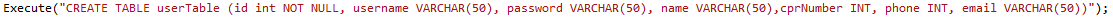
\includegraphics[width=16cm]{figures/SQLcreate.PNG}
\caption{SQL kommandoen der bliver benytte til at lave tabellen.}
\label{fig:sqlcreate}
\end{figure}

\subsection{Ordinal ranking}
Ordinal ranking er en måde at rangere objekter i forhold til hinanden. Hvis der f.eks. er 5 hold med følgende navne a1, a2, a3, a4 og a5, der har spillet en turnering, hvor a1 kom på første pladsen, a3 og a5 kom på anden pladsen, a2 kom på tredje pladsen og a4 kom på fjerde pladsen, så ville holdene blive rangeret således: 1: a1, 2: a3 eller a5, 3: a3 eller a5, 4: a2, 5: a4. Alle holdene bliver rangeret efter den plads de kommer på. Førstepladsen kommer først og sidstepladsen kommer sidst. De hold der så kommer på samme plads, som f.eks. a3 og a5, bliver så rangeret tilfældigt, medmindre de får en ekstra parameter som f.eks. at det hold der kommer først i alfabetet kommer først o.l. Et eksempel på en ordinal ranking rangering kan ses på figur \ref{fig:ranking} \citep{Cook1985, Cook1986}.

\begin{figure}[H]
\centering
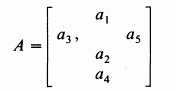
\includegraphics{figures/ranking.PNG}
\caption{Eksempel på en ordinal ranking opbygning.}
\label{fig:ranking}
\end{figure}

\subsection{Sikkerhed}
Sikkerhed af data er essentielt som udbyder af  software[kilde], \todo{mere text} 

\textbf{Passwords}
i software hvor passwords er userinput, er det vigtigt at de bliver holdt skjult, hvis fx. en hacker fik adgang til en af databaserne, hvor passwords bliver holdt, kunne personen bruge passwordsne til at komme dybere ind i systemet. Derfor benytter man sig af hashing. Et password der har været igennem en hashing algoritme bliver lavet til en hash-key, som ikke kan backtrackes til det originale password. Således gemmes kun det hashede password på databasen, sådan at hackeren der har fået adgang til databasen kun kan se hash key'et og ikke passwordsne. Det er essentielt at hashing algoritmen er en krævende proces, fordi den ellers er sårbar over for angrebsmetoder, der slavisk gennemgår alle mulige kombinationer indtil den finder en kode der bliver hashet til hash-keyet. 

\textbf{Hashing}
der findes flere forskellige hashing funktioner 

\subsection{Klient-Server struktur}
Der er to grunde til at løsningen splittes op til to stykker software.\todo{Mangler en forklaring på hvorfor vi har valgt at splitte softwaren op i to? -Smed} Den første af disse grunde er sikkerhed. Siden at brugeren af vores klient (kunden) skal kunne gemme medarbejdere, indstillinger m.m. skal klient delen af løsningen have forbindelse til et sted at gøre dette. For at det information kan gemmes, skal klienten sende SQL forespørgsler til en database. For at sikre kundens database skal deres klient ikke kunne sende SQL forespørgsler direkte til databasen. Første udkast til at indsætte en medarbejder i databasen ser således ud:

\begin{lstlisting}
String str = "INSERT INTO userTable (id, username [...] " + user.Email + "')";
\end{lstlisting}

Det er første og sidste del af den SQL forespørgsel der sætter en bruger ind. Hvis så den e-mail der sættes ind er: "bob@aau.dk", så ender variablen str med: "bob@aau.dk'". Hvis en bruger dog har onde intentioner og sætter e-mail til at være i første udkast af programmet:
\begin{lstlisting}
'bob'); DROP TABLE Users;
\end{lstlisting}

så slettes alle brugere der allerede findes. Hvilket på ingen måde er hensigtsmæssigt.

Af denne grund skal systemet have en server, hvor database input og output håndteres på. Så uanset hvad der forsøges, i forhold til at sætte ind i eller trække ud af databasen, bliver inputtet først kørt igennem serveren. Serveren har flere forskellige funktioner, der hver især er vigtige for enten programmets sikkerhed eller for at det kan køre generelt. Serverens funktioner, fra vigtigst til mindst vigtig (ment som at det skal virke).

\begin{enumerate}
    \item Fornuftighedskontrol af database input
    \item Gøre systemet allestedsnærværende
\end{enumerate}

Det første serveren skal gøre et at kontrollere input til databasen. Sådan at der ikke er nogen, der med onde intentioner eller bare ved uheld ødelægger databasen. Der er flere måder at udføre disse angreb, som er kaldt 'SQL Injections'. Et eksempel på sådan et angreb kan forkomme hvis brugeren har muligheden for at skrive forkert input, i f.eks. et log in system, hvor der bliver læst et brugernavn og et kodeord, kan en bruger med onde intentioner skriver '105 or 1=1', hvilket er tilsvarende til at noget altid er true (kan ses i figur \ref{fig:injection}). Dette kan give brugeren alt information om alle andre brugers, brugernavn og password. \citep{inject, TNSQLI}. Dette er kun et eksempel af mange SQL Injections. 

\begin{figure}[H]
\centering
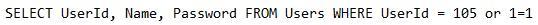
\includegraphics{figures/injection.PNG}
\caption{Eksempel på en '105 or 1=1' injection \citep{inject}.}
\label{fig:injection}
\end{figure}

Ud over det skal serveren give brugere af systemet muligheden for at tilgå systemet fra alle steder, hvor softwaren installeret. På den måde kan lederen lave ændringer hjemmefra, eller til møde osv. hvis han har softwaren eller en bærebar (med softwaren) med. Yderligere har det den effekt at, hvis en virksomheds computer udstyr bliver skiftet ud skal softwaren blot installeres på ny, så kan virksomheden fortsætte med at benytte systemet som de altid har gjort. Der skal ikke sættes indstillinger op igen, eller fumles rundt med versions kompatibilitet. Virksomheden kan bare benytte deres login så kan de benytte systemet. \\

\noindent\textbf{Simuleret Server}

Grundet budget og tid er det blevet vedtaget at der i stedet for en rigtig server bliver benyttet en simuleret server. Dette betyder at det software som kører vagtplanssystemet også kommer til at køre alt database arbejdet. Så det fra et programmerings perspektiv virker som om der er en server, uden at der faktisk er en.

\subsection{XAML}

XAML er en forkortelse for Extensible Application Markup Language. XAML er et XML baseret sprog. XML er en forkortelse for Extensible Markup Language. Et markup language er et sprog der bliver brugt til at behandle, definere og præsentere text \citep{Beal2015}. XML er et markup language der specifikt bliver brugt til at beskrive data. XML gør ikke noget af sig selv. For at kunne sende, modtage eller vise et XML dokument, så skal der skrives et stykke software til det \citep{W3C2015}. Selvom XAML er et XML baseret sprog gør de to sprog ikke det samme. Ethvert XAML dokument er et XML dokument, men et XML dokument kan ikke være et XAML dokument. XAML er et deklarativt applikation sprog, hvilket XML ikke er. Dette betyder at XAML i forhold til XML bruges til at beskrive objekter, ejendomme og deres forhold til hinanden \citep{T2009}.

\subsection{Testing}

Når et program bliver lavet, er der som regel brug for en metode til at finde ud af, om programmet virker optimalt. Der findes en række test metoder der kan bruges til dette formål. I projektet vil der blive kigget på følgende test metoder: Black Box Testing og White Box Testing.

\subsubsection{Black Box Testing}
Black box testing er en måde at teste et program på. Test metoden hedder Black Box Testing, fordi at programmet er for testpersonen ligesom en sort box, hvor vedkommende ikke kan se hvad der er indeni. Black Box Testing bliver som udgangspunkt foretaget af en bruger af programmet. Ved Black Box Testing, tester testpersonen programmet uden at vide hvad programmet indeholder. Et eksempel er en testperson der tester en hjemmeside ved at bruge en browser og derefter give input ved at klikke/skrive forskellige steder på hjemmesiden og verificere outputs og sammenligne dem med det forventede resultat. Black Box Testing modellen kan ses på figur \ref{fig:blackwhite}. Black Box Testing bruges til at finde fejl i følgende kategorier:\\

\begin{itemize}
\item{Inkorrekte eller manglende funktioner}.
\item{Interface fejl.}
\item{Fejl i datastrukturer eller ekstern database adgang.}
\item{Adfærd eller præstations fejl.}
\item{Initialisations og afslutnings fejl.}
\end{itemize}

Black box testing har en række fordele og ulemper. De lyder således:\\

\textbf{Fordele:} 
\begin{itemize}
\item{Testene bliver lavet som udgangspunkt lavet fra en brugers synspunkt, og hjælper derfor med at se hvordan eventuelle brugere ville forholde sig til det givne program, så programmet ikke kun bliver set gennem udviklernes øjne. Dette vil også hjælpe med at styr på uoverensstemmelser i en kravspecifikation.}
\item{Testpersonen har ikke behov for at kunne programmerings sproget bag programmet, eller hvordan programmet er blevet implementeret.}
\end{itemize}

\textbf{Ulemper:}
\begin{itemize}
\item{Kun et minimum antal af inputs kan blive testet og mange programveje vil forblive uprøvede.}
\item{det kan være svært at designe en test case uden klare specifikationer.}
\end{itemize}
\citep{Fundamentals2010}

\subsubsection{White Box Testing}

White box testing er en måde hvor man kan teste et program på. Metoden hedder White Box Testing fordi at programmet er for brugeren ligesom en hvid/klar box, hvor man kan se hvad der er indeni. White box testing bliver også tit refereret som f.eks. Glass Box Testing eller Open Box Testing. Ved White Box Testing ved testpersonen som udgangspunkt alt om programmet og hvad det indeholder. Denne test bliver som udgangspunkt udført af udvikleren. Et eksempel på White Box Test kan være således: Testpersonen studerer implementationen af en kode af et bestemt område af en hjemmeside, hvor testpersonen bestemmer gyldige og ugyldige og ulovlige inputs og verificerer outputs og sammenligner dem med det forventede resultat. White Box Testing modellen kan ses på figur \ref{fig:blackwhite}. White Box Testing bruges til at finde fejl i følgende kategorier \cite{Guru992015}:

\begin{itemize}
\item{Interne sikkerhedshuller.}
\item{Brudte eller dårligt konstruerede veje i kodnings processen.}
\item{Kodens flow for specifikke input.}
\item{Funktionaliteten af loops.}
\item{Test af hvert statement, object og funktion på et individuelt basis.}
\end{itemize}

White Box Testing har en række fordele og ulemper. De lyder således:\\

\textbf{Fordele:}

\begin{itemize}
\item{Hjælper med at optimere koden.}
\item{Hjælper med at fjerne de ekstra linjer af kode som kan føre til defekter.}
\item{Testen er mere grundig.}
\end{itemize}
\citep{Prasad2008}

\textbf{Ulemper:}

\begin{itemize}
\item{Testene kan være meget komplekse, så der er brug for mange og dygtige ressourcer, hvilket kan være dyrt.}
\item{Som udgangspunkt så kan en White Box Test ikke blive lavet uden at modificere i programmet der testes.}
\item{Tager lang tid at teste alle mulige output af et program.}
\end{itemize}
\citep{Prasad2008}
\citep{Fundamentals2010White}

\begin{figure}[H]
\centering
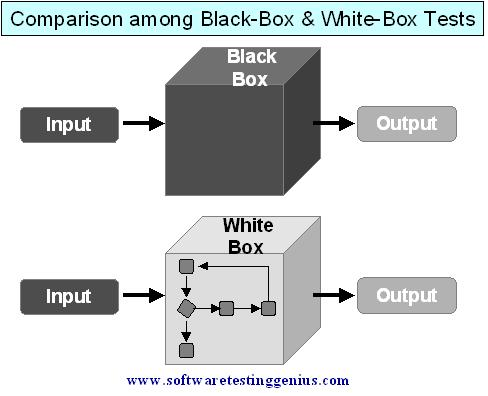
\includegraphics[scale=0.75]{figures/blackwhite.PNG}
\caption{En model der viser hvordan de to box testing metoder virker og deres forskelle \citep{Genius2015}.}
\label{fig:blackwhite}
\end{figure}

I dette projekt vil både White Box Testing og Black Box Testing blive brugt. White Box Testing vil bruges til Unit Testing og Integration Testing. Herefter vil Black Box Testing blive brugt til System Testing og Acceptance Testing. De fire tests rækkefølge i forhold til hinanden kan ses på figur \ref{fig:test1}. Det er ikke nødvendigt at køre sit program gennem alle fire tests, dog er det det mest hensigtmæssige i forhold til hvis der ønskes det mest fejlfrie program.

\subsubsection{Unit Testing} \label{test}

Unit Testing er en måde at bruge White Box Testing på. I Unit Testing testes individuelle units/komponenter af et program. Dette gøres med henblik på at validere at alle units agerer på den måde som de er designet til. Et unit er den mindste del af et program som er testbart. Et unit har som udgangspunkt et eller et par inputs og som udgangspunkt ét output. I objektorienteret programmering er den mindst testbare unit en metode. Unit Testings plads i testing kan ses på figur \ref{fig:test1}. Unit Testing er den første del af testing. Unit Testing bliver udført før Integration Testing. Unit Testing bliver som udgangspunkt lavet af det givne programs udviklere. Unit Testing processen har ni stadier, fire i Unit Test Plan, fire i Unit Test Cases Script, og et i den afsluttende Unit Test.

\textbf{Unit Test Plan:} Denne del omhandler den plan der bliver for den Unit Testing der skal udføres.

\begin{itemize}
\item{\textbf{Prepare}}
\item{\textbf{Review}}
\item{\textbf{Rework}}
\item{\textbf{Baseline}}
\end{itemize}

\textbf{Unit Testing Cases:} Denne del omhandler hvordan der forholdes til de forskellige dele der skal testes.

\begin{itemize}
\item{\textbf{Prepare}}
\item{\textbf{Review}}
\item{\textbf{Rework}}
\item{\textbf{Baseline}}
\end{itemize}

\textbf{Unit Testing:} Denne del omhandler den sidste del af Unit Testen, hvor der ses hvordan programmet klarer sig.

\begin{itemize}
\item{\textbf{Perform}}
\end{itemize}

\citep{Fundamentals2011}.

\subsubsection{Integration Testing}

Efter en Unit Test er blevet lavet, så er det mest hensigtmæssige valg at lave en Integration Test. Både White Box Testing og Black Box Testing kan som udgangspunkt bruges til Integration Test. Integration Test er en test hvor de individuelle units bliver testet sammen som en gruppe. Integration Testing laves med henblik på at finde fejl når programmets units interagerer med hinanden. Integration Testings plads i testing processen kan ses på figur \ref{fig:test1}. Integration Testing er den anden del i testing. Den bliver udført før System Testing. Ligesom Unit Testing så bliver Integration Testing som udgangspunkt lavet af det givne programs udviklere. Integration Testing processen har de samme stadier som Unit Testing processen som kan ses i afsnit \ref{test} \citep{Fundamentals2011Integration}.

\subsubsection{System Testing}

Næste led efter Integrations Testing er System Testing. System Testing er en test hvor det fuldendte program bliver testet. Til System Testing bruges Black Box Testing som udgangspunkt. Målet med System Testing er at evaluere det givne programs kompilering med programmets specifikke krav. System Testings plads i testing processen kan ses på figur \ref{fig:test1}. System Testing er den tredje del i testing. Den bliver udført før Acceptance Testing. Denne test bliver til forskel fra Unit og Integration Tests lavet af en bruger/tester. System Testing processen har de samme stadier som Unit Testing processen som kan ses i afsnit \ref{test} \citep{Fundamentals2011System}.

\subsubsection{Acceptance Testing}

Efter System Testing så kommer Acceptance Testing. I dette led bliver det givne testet for acceptabilitet. Til Acceptance Testing bruges Black Box Testing som udgangspunkt. Målet med denne test er at evaluere programmets kompilering med udviklernes krav og brugernes vurdering, og finde ud af om programmet er acceptabelt nok til levering. Acceptance Testings plads kan ses på figur \ref{fig:test1}. Acceptance Testing er den anden del i testing. Den bliver udført til sidst. Acceptance Testing bliver ligesom System Testing lavet af en bruger/tester. Acceptance Testing processen har de samme stadier som Unit Testing processen som kan ses i afsnit \ref{test} \citep{Fundamentals2011Acceptance}.

\begin{figure}[H]
\centering
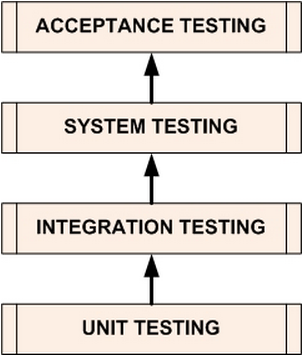
\includegraphics[scale=0.5]{figures/test1.PNG}
\caption{En model der viser hvilken rækkefølge de fire tests: Unit Testing, Integration Testing, System Testing og Acceptance Testing kommer i \citep{Fundamentals2011Testing}.}
\label{fig:test1}
\end{figure}

\subsection{Flowcharts}

Flowcharts er en måde hvor man kan visualisere en proces ved hjælp af en række logiske sekvenser. Det er også en måde hvorpå en program struktur kan organiseres og gøres mere læsbar for en bruger. Flowcharts bruger simple geometriske symboler og pile til at definere forhold imellem et givet programs dele. I programmering bruges disse symboler:

\begin{itemize}
\item{\textbf{Oval:} Bruges til at repræsentere starten og slutningen af et program.}
\item{\textbf{Rektangel:} Bruges til at repræsenter en proces.}
\item{\textbf{Diamant:} Bruges til at repræsentere et valg.}
\item{\textbf{Parallelogram:} Bruges til at repræsentere én input/output proces.}
\end{itemize}
\citep{Rouse2008}

Et eksempel på et flowchart diagram kan ses på figur \ref{fig:flowchart}.

\begin{figure}[H]
\centering
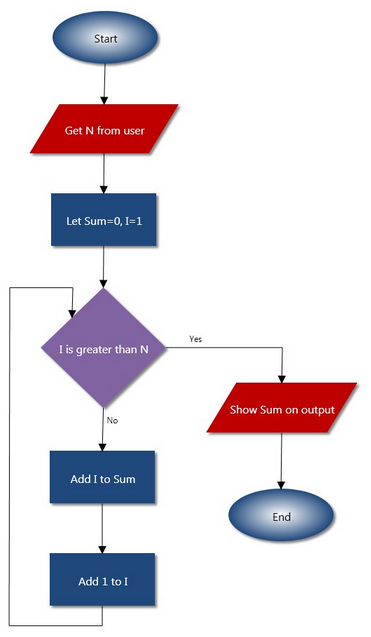
\includegraphics[scale=0.75]{figures/flowchart.PNG}
\caption{Et eksempel på et flowchart diagram, som de bliver brugt i programmering \citep{Barahimi2013}.}
\label{fig:flowchart}
\end{figure}

\citep{Network2015}
